\chapter{Auswertung}
Im letzten Teil dieser Arbeit wird das Huff-Modell und dessen Umsetzung im Prototypen ausgewertet.\\
Was sind die Anwendungsfälle des Huff-Modells?
Wozu kann der Prototyp verwendet werden?
Ist der Prototyp performant?
Ist das Huff-Modell eine gute Wahl für einen Algorithmus der Filialplanung und Standortanalyse?
Wo stößt das Modell an seine Grenzen?
Was kann verbessert, erweitert oder ersetzt werden?

Unter anderem diesen Fragen wird mit Ausblick auf die Zukunft kritisch Antwort gegeben bevor ein finales Fazit gezogen wird.

\section{Bewertung}
\label{sec:bewertung}
Bei der Bewertung des Prototypen muss einerseits die Umsetzung des Huff-Modells in einer Webkarte mit modernen Technologien und andererseits das Modell selber bewertet werden.
Hierzu werden zunächst Anwendungsfälle des Modells beschrieben, die Verwendung des Prototypen unter Einbeziehung der Performance für diese erklärt und Verbesserungen und Erweiterungen vorgestellt.
Danach wird das Modell selber in Frage gestellt und mögliche Alternativen oder Erweiterungen vorgestellt.

Obwohl das Huff-Modell kein neues Phänomen und schon mehrere Jahrzehnte alt ist, hat es sich als verlässlich erwiesen und findet nach wie vor Gebrauch.
Die liegt vor allem an der einfachen und schnellen Verwendung. 
Bereits mit wenig Informationen können simple Prognosen zu Besucherwahrscheinlichkeit erstellt werden.\\
Zu den Hauptanwendungsfällen zählen:

\begin{itemize}
	\item Filialplanung
	\item Expansionsplanung
	\item Verteilgebietsplanung
	\item Kundenansprache
\end{itemize}

Die Filialplanung und Expansionsplanung sowie die Verteilgebietsplanung und die Kundenansprache sind ähnlich zu betrachten, da sie sich nur geringfügig unterscheiden.\\
Der Prototyp kann alle aufgelisteten Fälle grundlegend abdecken, könnte aber aber bei gezielten Erweiterungen eine noch bessere Unterstützung für die spezifischen Anforderungen bieten.
So lassen sich Besuchswahrscheinlichkeiten in bestehendem Netz sowie mit neuen Filialen berechnen und vergleichen.
Potenzielle neue Standorte können dem bestehenden Netz hinzugefügt werden und deren Auswirkung auf Wahrscheinlichkeiten und Umsatz werden direkt visuell und numerisch sichtbar, was bei direktem Vergleich die Erstellung einer Reihenfolge anhand von Umsatzgewinn oder -verlust und Marktanteil der potenziellen neuen Standorte erlaubt.\\ 

Ebenso kann sehr leicht ein Verteilgebiet für Handzettel (Werbung) abgegrenzt werden, dass sich auch wirklich nur an Kunden richtet, die wahrscheinlich in der Filiale einkaufen würden.
Außerdem sind aus den Gebieten des Verteilgebiets erste Informationen zu Kaufkraft, Einwohneranzahl und Ausgaben ersichtlich, was eine persönlichere Ansprache der Kunden zulässt, die auf demografischen Analysen beruht.\\
Eine sinnvolle Erweiterung für die Verteilgebietserstellung wäre die Gruppierung mehrerer Gebiete zu einem neuen Verteilgebiet in einem neuen Layer.
Das neue Gebiet könnte dann eine eigene Farbe erhalten und nach Bedarf ein- und ausgeblendet werden oder in der Z-Ebene nach oben oder unten verschoben werden.
Für das neue Gebiet können dann die Daten der eingeschlossenen Gebiete summiert werden und für das potenzielle Verteilgebiet angezeigt werden.

Die Berechnung des Modells ist bereits angemessen performant mit initialer Lade- und Renderzeit von unter 1 Sekunde für die Gebiete und Filialen sowie Berechnungs- und Rerenderzeit der Gebiete von ebenfalls unter 1 Sekunde.
Durch Optimierung beim Laden und Rendern durch zum Beispiel explizite Nutzung von Cache-Objekten für Features und Styles oder Überarbeitung des Codes für die Berechnung des Modells könnte hier eventuell noch eine bessere Performance erzielt werden

Der Prototyp kann das Huff-Modell sehr gut darstellen und bietet echten Mehrwert in Prozessen des Geomarketings.
Dennoch hat das Modell auch einige Schwächen oder Ungenauigkeiten, wie unter anderem bereits im Artikel \glqq Application of network Huff model for commercial network planning at suburban – Taking Wujin district, Changzhou as a case\glqq von Haozhi Pan,Yongfu Li und Anrong Dang beschrieben \footcite{pan_application_2013}.
Die Autoren bezeichnen vor allem die Bestimmung der Parameter $\alpha$ und $\beta$ sowie die Berechnung der Distanzvariable D als problematisch.
Während es für die Bestimmung der Parameter meist an regionalen Marktdaten mangelt oder eine Regressionsanalyse mit Linearisierung oder Ähnliche  nur schwer durchzuführen ist, gibt es schlicht mehrere Möglichkeiten die Distanz zwischen Filiale und Kunde zu berechnen.
Die Distanz kann euklidisch dargestellt werden oder über die Netzwerkdistanz oder - zeit (Fahrzeitzone in Meter oder Minuten), wobei alle drei zu verschiedenen Ergebnissen des Modell führen.\\
Des Weiteren benutzt das Huff-Modell nur genau zwei Variablen(A und D), die über die Kundenentscheidung des Besuchs entscheiden sollen.
Aufgrund dieser Einschränkung und den bereits aufgeführten Problemen in Bezug auf die Bestimmung der Parameter $\alpha$ und $\beta$ war das Huff-Modell im Laufe der Jahre bereits mehrfach Kern wissenschaftlicher Arbeiten, die sich mit der Validierung und Verbesserung des Modells beschäftigten.\\
Daraus entstand 1974 das (erste \footnote{Es folgten weitere Erweiterungen auf Basis von MCI}) Multiplicative Competitive Interaction Modell (kurz MCI-Modell) entwickelt von Masao Nakanishi und Lee Cooper, welches genau diese Probleme behandeln sollte und eine Bestimmung der Parameter über mathematische Verfahren wie zum Beispiel die (gewöhnliche) Methode der kleinsten Quadrate ermöglichte \footcite{nakanishi_parameter_1974}. 
Weitere wissenschaftliche Modelle sind das Multiple Store Location Model von Dale Achabal \footcite{achabal_slop_1984} oder ein verallgemeinertes Huff-Modell von Daniel Griffith \footcite{griffith_generalized_1982}.
Die Attraktivität einer Filiale hängt von deutlich mehr Faktoren als nur der Größe und Anzahl der Parkplätze ab.
Markenstärke, Sortiment und Preise beeinflussen ebenfalls in die Entscheidung des Kunden, um nur ein paar weitere Faktoren zu nennen.
Um diese Faktoren in die Berechnung mit einfließen zu lassen und eine lineare Formel für die Berechnung zu erhalten, verwendet das MCI-Modell folgende Erweiterung der Huff-Modell-Formel:

\begin{equation}
	P_{i j}=\left(\prod_{h=1}^{H} A_{h j}^{\gamma_{h}}\right) D_{i j}^{\lambda} / \sum_{j=1}^{n}\left(\prod_{h=1}^{H} A_{h j}^{\gamma_{h}}\right) D_{i j}^{\lambda}
\end{equation}

Dabei gilt:

\begin{tabbing}
	\( P_{i j} \) \= = die Wahrscheinlichkeit, mit der Kunde j in Filiale i einkauft;\\
	\( A_{h j} \) \> = ein Maß der h Eigenschaften (h = 1,2,.H), die die Attraktivität der Filiale j angeben;\\
	\( \gamma \) \> = ein Parameter der Sensibilität von \(P_{i j}\) in Verbindung mit einer Attraktionsvariable h;\\
	\( D_{i j}^{\lambda} \)	\> = ein Maß der Erreichbarkeit der Filiale j für einen Kunden i;\\
	\( {\lambda} \)	\> = ein Parameter der Sensibilität von \(P_{i j}\) in Verbindung der Erreichbarkeit;\\
	n \> = die Anzahl der Filialen.
\end{tabbing}

Huff selber veröffentlichte diese Formel 2008 in einem Artikel, in dem er die Problematiken des ursprünglichen Modells erläutert und auf die Verbesserungen eingeht und ein Kalibrierung des Modells vorstellt \footcite{huff_calibrating_2008}.

Ebenso finden sich auch direkt im Prototypen einige Schwächen.\\
So lassen sich Filialen finden, bei denen die Berechnung zu einem ungenauen Ergebnis führt, wie in Abbildung \ref{img:innacc_store} zu sehen.
In der Abbildung ist klar zu erkennen, dass das Gebiet in welchem sich die Filiale befindet selbst nicht die höchste Besuchswahrscheinlichkeit hat.
Diese Ungenauigkeit lässt sich auf die Berechnung des Mittelpunkts des Gebiets zurückführen.
So ist die Filiale näher am Mittelpunkt des Nachbargebiets als am Mittelpunkt des eigenen Gebiets gelegen, was zu einer höheren Besuchswahrscheinlichkeit des Nachbargebiets führt.\\
Dieses Problem lässt sich relativ einfach mit der Verwendung von kleineren Gebieten eindämmen.
Jedoch ist die ideale Lösung mit der Verwendung von Punkten pro Haushalten nicht wirklich umsetzbar, da die Datenmenge um ein Vielfaches größer wäre und die Berechnung zu viel Ressourcen benötigen oder zu lange dauern würde.

\begin{figure}[H]
	\makebox[\textwidth][c]{
		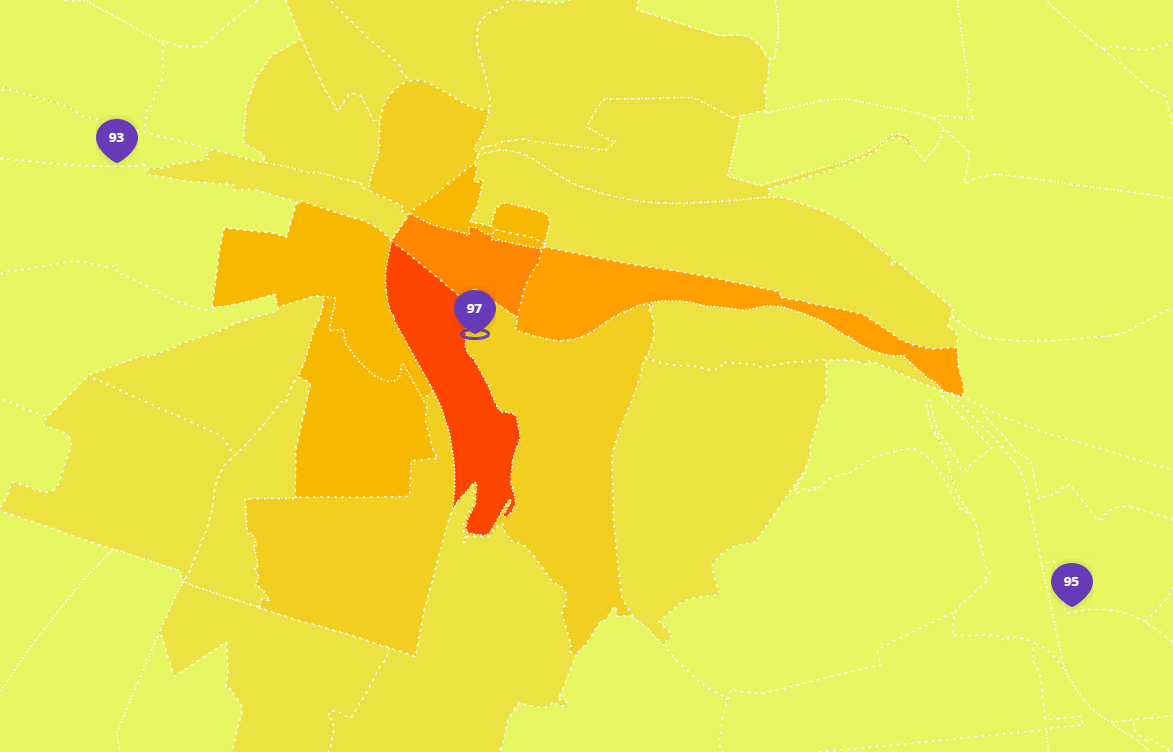
\includegraphics[scale=0.4]{resources/images/ungenaue_filiale.png}}
	\caption{Bildschirmausschnitt des Prototypen mit ungenauer Berechnung}
	\label{img:innacc_store}
\end{figure}


\section{Fazit/ Ausblick}
Das Huff-Modell als Grundlage der algorithmischen Berechnung in dem Prozess einer Filialplanung erweist sich als einfach zu verstehendes, schnelles und nützliches Werkzeug, um mit relativ wenig Marktdaten bereits eindeutige und aussagekräftige Informationen über mögliche neue Standorte einer Filiale zu erhalten.\\
Im Prototypen wurden die verfügbaren Marktdaten um lediglich ein paar wenige Attribute ergänzt, um eine realistische Abbildung eines Filialnetzes innerhalb Berlins zu generieren. 
Um die Berechnung komplexer und somit hoffentlich genauer erfolgen zu lassen, ist eine Erweiterung des Huff-Modells wie in \ref{sec:bewertung} beschrieben denkbar.
Die Parameter der Berechnung sollten sich dann einfach fast beliebig erweitern lassen, so können in die Berechnung der Attraktivität deutlich mehr Attribute einer Filiale oder des Umfelds einfließen.
Denkbar sind zum Beispiel die Ergänzung von Informationen über umliegende Sehenswürdigkeiten (engl. Point of interest), die Eingliederung der Filiale in ein Einkaufszentrum, Markenstärke einer Filialkette oder tatsächliches Sortiment.
Sie alle nehmen Einfluss auf die Attraktivität einer Filiale.\\
Ebenso kann die Berechnung der Distanz auf komplexeren Grundlagen wie zum Beispiel der Fahrzeit mit dem Auto, den öffentlichen Verkehrsmitteln oder dem Fahrrad basieren.\\
Auf die Notwendigkeit der Bestimmung der Parameter $\alpha$ und $\beta$ wurde bereist im Kapitel \ref{ch:implementierung} \glqq Implementierung\glqq eingegangen.
Kundenbefragungen, amtliche Statistiken oder Meinungsbilder können hier als Grundlage dienen, um die Parameter zu bestimmen.\\
Für die Anwendung in echten Szenarien der freien Wirtschaft sollte also unbedingt eine verfeinerte Kalibrierung der Berechnung anhand eigener Daten erfolgen, damit der Prototyp mit vollem Potenzial verwendet werden kann.\\
Außerdem wäre eine Erweiterung hinsichtlich direkter Gegenüberstellung der potenziellen Standorte in Form einer Tabelle oder Ähnlichem denkbar.
Im Prototyp lassen sich zwar beliebig viele neue Filialen setzen, jedoch gibt es keine Möglichkeit die gesetzten Filialen und deren Einfluss auf Wahrscheinlichkeiten und Marktanteil zu vergleichen.\\
Die Darstellung der Gravitationsebenen erfolgt im Prototypen über die Einfärbung der Gebiete.
Eine detaillierte Darstellung direkt über Isolinien der Wahrscheinlichkeit wäre unter Verwendung einer Geometriefunktion und Stylefunktion möglich. 
So müssten aus den Isolinien neue Polygone erstellt werden und diese anhand der Ebene entsprechend eingefärbt werden.

Als Komponente eines größeren, komplexeren GIS würde der Prototyp einzigartige, ergänzende Features bieten, die die Prozesse innerhalb der Standortanalyse und Filialplanung deutlich vereinfachen.
Obwohl das Huff-Modell im Laufe der Jahre oft erweitert wurde, führt es in seiner Grundfunktion bereits zu aussagekräftigen Ergebnissen.
Sicherlich können diese Ergebnisse über erwähnte Erweiterungen verbessert und verfeinert werden, jedoch steigt damit auch die Komplexität des Modells und schränkt im Zweifel die allgemeine Anwendung auf spezielle Anwendungsfälle ein.\\
Somit bleibt festzuhalten: Durch niedrige Komplexität, vielfältige   Anwendungsbereiche und eine schnelle, simple Umsetzung bietet sich das Huff-Modell gut für die Anwendung im Prozess der Standortanalyse und Filialplanung an.